\documentclass{article}

\title{Research Report}
\author{Daan de Jong}
\date{October 2020}

\usepackage{setspace}\onehalfspacing
\usepackage[a4paper]{geometry}
\usepackage{graphicx}
\usepackage{apacite}
\graphicspath{ {./img/} }
\usepackage{caption}
\usepackage{subcaption}
\usepackage{natbib}
\usepackage{amsmath}
\usepackage{amssymb}
\usepackage{multirow}

\usepackage{sectsty}
\sectionfont{\large \centering}
\subsectionfont{\small}
\subsubsectionfont{\small}
\paragraphfont{\large}

\usepackage{fancyhdr}
\fancyhead[L]{Research Report}
\fancyfoot[C]{\thepage}

\usepackage{multicol}
\setlength{\columnsep}{1cm}

\begin{document}

\begin{titlepage}
	\begin{center}
		\vspace*{2cm}

		\Huge
		\textbf{Research Report}
		
		\Large
		\textbf{Negation Scope Detection with LSTM Neural Networks}
		
		\vspace{1.5cm}
		
		\textbf{Daan de Jong}
		
		5942713

		
\includegraphics{UU}
			
		\vfill
					
		\large
		
		Faculty of Social and Behavioral Science\\
		Department of Methodology and Statistics\\
		Study programme: MSBBSS\\
		Supervisor: dr. Ayoub Bagheri\\
	
			
	\end{center}


\end{titlepage}

\pagestyle{fancy}

\begin{multicols}{2}

\section{Introduction}

Negation is a complex grammatical phenomenon that has been widely studied by disciplines as philosophy, cognitive science and linguistics \citep{modality-and-negation}. Within the field of Natural Language Processing (NLP), it plays an important role in the semantic representation of text and has received considerable attention in recent years \citep{SEM-shared-task}. 

A negation can be defined as ``the implication of the non-existence of something'' \citep{bioscope} or ``a grammatical category that comprises devices used to reverse the truth value of propositions'' \citep{SEM-shared-task}. It is useful to make a distinction between the \textit{cue} and the \textit{scope} of a negative instance. A negation cue is a word, a morpheme or a group of words that inherently expresses a negation, for example, `never', `impossible' or `not at all'. Its negation scope comprises the elements of the text that are affected by it. Consider the following example, where the negation cue is boldfaced and the negation cue is enclosed by square brackets:

\begin{center}
That's [\textbf{not} a problem \textbf{at all}.]
\end{center}

Note that the negation cue can be discontinuous, and that it is annotated as a part of its scope.

The current report will focus on detection of negation scopes. When the goal is to derive factual knowledge from textual data, it is important that negation scopes are resolved correctly, given the fact that their meaning is altered by their negation cue. Moreover, negations are reasonably common, with a frequency of 27.6 per 1,000 words in spoken text and 12.8 per 1,000 words in written text \citep{tottie}. So, typical NLP tasks might benefit from adequate tools to handle negations.

Earlier efforts to detect the scope of negations in natural language can be categorized into rule-based approaches \citep[e.g.][]{basile2012ugroningen, ozgur-radev-2009-detecting, ovrelid-2010} and statistical learning methods \citep[e.g.][]{fei2020negation, zou-etal-2013-tree, tang-etal-2010-cascade}. In both of these categories, models or systems for negation scope detection have performed considerably well. However, they need human-engineered features to reach this performance. 

To overcome the need of manually-crafted features researchers have proposed Neural Network-based approaches for the task of negation scope detection, since these kind of models are able to learn unsupervised features from the data. For example, \cite{qian-2016} used a Convolutional Neural Network-based model to extract path features from syntactic trees and combined these with position features to resolve the negation scope. As an alternative, \cite{sergeeva2019} proposed a Recurrent Neural Network-based approach that utilizes unsupervised word-embeddings and character-level word-embeddings with pre-computed syntactic features as inputs for a bidirectional Long Short-Term Memory (BiLSTM)-layer. The bidirectional character of this layer ensures that negation scope parts located at both sides of the negation cue can be captured. A similar approach was adopted by \cite{fancellu2016neural}, who evaluated a BiLSTM-based approach in comparison to a feed forward Neural Network model, that both integrated pre-specified information about the negation cue and part-of-speech (PoS) tags. All of these models perform at a state-of-the-art level.

Based on the BiLSTM-model proposed by \cite{fancellu2016neural}, the current study adopts a BiLSTM-approach with sentence and cue embedding inputs to perform the task of negation scope detection on biomedical text data, with the following contributions: (i) In contrast to \cite{fancellu2016neural}, both negated and non-negated sentences are used to train this model, to expose the model to a more natural set of data. (ii) The model is trained on text data from another genre. (iii) The model is slightly extended with an additional dense layer after the LSTM-layers. (iv) Furthermore, the current study tries to handle the problem described by \cite{fancellu2017detecting}, who suggested that negation scope detection models might overfit negation scopes that are enclosed by punctuation marks. To this end, punctuation marks are excluded in the tokenization process. In this way, this study expands the knowledge about how Neural Networks can be used to automatically resolve negation scopes in natural language, that is, without reliance on manually-crafted features.

This report should be read as a intermediate documentation of the current study. In the Methods section, the basic model architecture and data flow are described. The Results section reports on the performance of this model in one specific setting of hyperparameters. In the Discussion section, possible ways to extend the current study are considered.

\section{Methods}

\subsection{Data}
The current study made use of the biological full papers and biological scientific abstracts subcorpora from the freely available BioScope corpus \citep{bioscope}. In this corpus, negative keywords and their linguistic scope are annotated for each sentence. These annotions were carried out such that the set of keywords in a sentence is as small as possible, and the corresponding scope is as wide as possible. This results in the fact that none of the negation scopes are discontinuous. A small description of the data set is provided in Table \ref{datadescription}. 

\begin{table*}[t]
	\centering
	\caption{Descriptives of the corpora.}
	\label{datadescription}
	\begin{tabular}{l | c c | c}
	\hline
	 & Abstracts & Full Papers & Total \\
	\hline \hline
	\# Sentences & 11993 & 2469 & 14462\\
	\# Negation instances & 1719 & 375 & 2094 \\
	\% Negation instances & 14.3 & 15.2 & 14.5 \\
	\hline
	\end{tabular}
\end{table*}

\subsection{Data preprocessing}
The data set consists of 14462 sentences with their negation cue and negation scope annotations. After standardization and tokenization, a sentence $s_i$ is represented by a vector $\mathbf{x}_i = (x_{1_i}~\cdots~x_{t_i}~\cdots~x_{n_i})^{\prime}$ of tokens, where $i$ is the sentence index, $n_i$ is the number of tokens in the sentence and $t = 1,2, \dots, n$ is its token index. In the current study, hyphenated words were considered as one token, and commas and periods were excluded. This resulted in 17602 unique tokens. Let the vocabulary $X = \{x_1,\dots, x_{17602}\}$ be the ordered set of tokens and $V=\{1,\dots,|X|\}$ the set of their indices, so that every token is associated with a unique vocabulary index in V. Then, a token vector $\mathbf{x}_i$ can be vectorized by mapping each $x_{t_i}$ to its vocabulary index $v_{t_i} \in V$, obtaining a sequence $\mathbf{v}_i = (v_{1_i}~\cdots~v_{n_i})^{\prime}$ for each sentence $s_i$.

Each sentence $s_i$ is associated with a negation cue vector and a negation scope vector. The cue vector $\mathbf{c}_i = (c_{1_i}~\cdots~c_{n_i})^{\prime} \in \{0,1\}^{n_i}$ indicates which tokens are annotated as a cue token, so $c_{t_i}=1$ if the $t$-th token from the corresponding token vector $\mathbf{x}_i$ is a negation cue and $c_{t_i}=0$ otherwise. The scope vector of sentence $s_i$ is defined as $\mathbf{y}_i=(y_{1_i}~\cdots~y_{n_i})^{\prime} \in \{0,1\}^{n_i}$, where $y_{t_i}=1$ if the $t$-th token from $\mathbf{x}_i$ is annotated as a negation cue or affected by it, and $y_{t_i}=0$ otherwise. This vector is referred to as the label vector.

The average length of a sentence was 23.67 tokens and the average scope length\footnote{average scope length of scopes that were longer than zero} was 8.38 tokens, where the scope length of $\mathbf{y}_i$ is defined as $\sum_{t=1}^{n} y_{t_i}$. For model training, 11500 randomly selected (sequence, cue, label)-triples were used, which corresponds to about 80\% of the data. The remaining triples were used for testing.

\subsection{Task modeling} 
The task is to predict the label vector $\mathbf{y}_i$ given $\mathbf{v}_i$ and $\mathbf{c}_i$. As an example from the data set, sentence $s_{169}$,

\begin{center}
\textit{This element has no activity in T cells of the Jurkat line},
\end{center}

is labeled as

\begin{center}
\textit{This/0 element/0 has/0 no/1 activity/1 in/1 T/1 cells/1 of/1 the/1 Jurkat/1 line/1.}
\end{center}

So, the task in this example is to predict $\mathbf{y}_{169}=(0~0~0~1~1~1~1~1~1~1~1~1)^{\prime}$ given $\mathbf{v}_{169}=(24~90~75~114~36~3~21~8~2~1~177~122)^{\prime}$ and $\mathbf{c}_{169}=(0~0~0~1~0~0~0~0~0~0~0~0)^{\prime}.$ To this end, each token is given a predicted probability that it is inside the negation scope. These probabilities are then concatenated into a single vector to predict the label vector. 

\begin{center}
\captionsetup{type=figure}
	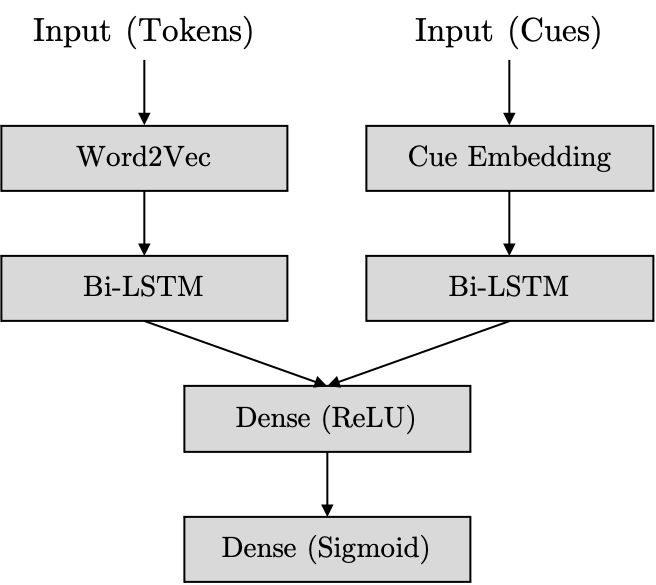
\includegraphics[scale=0.5]{model2}
	\caption{Schematic representation of the model.}
	\label{modelfigure}
\end{center}

\subsection{Model architecture}
Negation scope classification for each sentence was performed by a neural network consisting of an embedding layer, a BiLSTM layer and two dense layers. As inputs, the model takes a sequence $\mathbf{y}_i$ and its corresponding cue vector $\mathbf{c}_i$. These are fed into their own embedding layer and BiLSTM layer, subsequently concatenated, fed through a dense layer with a ReLU activation and finally into another dense layer, the output layer, see Figure \ref{modelfigure}. The values from the output layer can be interpreted as the probability for each token of being part of the negation scope. The following subsubsections describe how a sequence $\mathbf{v}$ and a cue vector $\mathbf{c}$ are processed through the layers of the model\footnote{For clarity, the subscript $i$ will be omitted in this section.}. \newline

\textit{Embedding layers}.
Within a sequence $\mathbf{v}$, a 50-dimensional word embedding $\mathbf{e}_t \in \mathbb{R}^{50}$ is obtained for each $v_{t}$ using a Word2Vec model \citep{word2vec}. Word embeddings were trained on the entire data set with the skip-gram algorithm, where the task is to correctly identify the context word of a target word from a set of random negative samples and the true context word. Here, a context window size of 5 and a negative sample size of 15 were used. An embedded sentence can then be represented as a $d \times n$ matrix $E = (\mathbf{e}_{1}~\cdots~\mathbf{e}_{n})$. Word embeddings were not updated during training of the model on the negation scope detection task.

For each $c_t$ within a cue vector $\mathbf{c}= (c_1~\cdots~c_{n})^{\prime}$, the cue embedding layer yields a cue embedding $\mathbf{q}_t \in \{1\}^{50}$ if $c_{t}=1$ and $\{0\}^{50}$ if $c_{t}=0$. Then, the cue embedding of sentence $s$ can be represented as a $d \times n$ matrix $Q = (\mathbf{q}_{1}~\cdots~\mathbf{q}_{n})$. The cue embedding layer was specified to be non-trainable, since the cue embeddings should function in the same way for each $\mathbf{c}$. \newline 

\textit{BiLSTM layers}.
The embedded sentence $E$ and the embedded negation cue $Q$ are passed to their own BiLSTM layer \citep{hochreiter}. Both layers consist of 64 units: 32 units in the forward direction where the time-step $t$ moves from 1 to $n$ and 32 units in the backward direction where $t$ moves from $n$ to 1. Time-step $t$ corresponds to the $t$-th column of the input matrix. In this subsection, only the BiLSTM layer with input $E$ will be discussed, since the layer with input $Q$ is designed identically. 

Let $\mathbf{i}_t, \mathbf{f}_t, \mathbf{o}_t$ and $\mathbf{h}_t$ denote the input gate, forget gate, output gate and hidden layer state of the LSTM-cell, respectively, at time-step $t$. Let $W_e$ denote the weight matrices of the embedding input and $W_h$ the weight matrices of the previous hidden state, and let superscripts $(i), (f)$ and $(o)$ indicate to which gate the matrix belongs. Let $\mathbf{b}$ be the bias vectors with similar superscripts. Then the input, forget and output gate of the BiLSTM layer can be described as 

$$
\begin{aligned}
\mathbf{i}_t &= \sigma\big(W_e^{(i)}\mathbf{e}_t + 
W_h^{(i)}\mathbf{h}_{t-1} +\mathbf{b}^{(i)} \big), \\ 
\mathbf{f}_t &= \sigma\big(W_e^{(f)}\mathbf{e}_t + 
W_h^{(f)}\mathbf{h}_{t-1} +\mathbf{b}^{(f)} \big), \\
\mathbf{o}_t &= \sigma\big(W_e^{(o)}\mathbf{e}_t + 
W_h^{(o)}\mathbf{h}_{t-1} +\mathbf{b}^{(o)} \big), \\ 
\end{aligned}
$$

where the sigmoid function $\sigma: \mathbb{R}\rightarrow(0,1)$ is given by $x \mapsto \frac{1}{1+e^{-x}}$. 

The cell state $\boldsymbol{\gamma}$ at time-step $t$ is a combination of the previous cell state $\boldsymbol{\gamma}_{t-1}$ and the candidate cell state $\tilde{\boldsymbol{\gamma}}$: $$\boldsymbol{\gamma}_t=\mathbf{f}_t * \boldsymbol{\gamma}_{t-1} + \mathbf{i}_t * \tilde{\boldsymbol{\gamma}}_{t},$$ where `$*$' denotes element-wise multiplication and the candidate cell state is defined as $$\tilde{\boldsymbol{\gamma}}_t=\mathrm{tanh}(W_e^{(\tilde{\boldsymbol{\gamma}})}\mathbf{e}_t + W_h^{(\tilde{\boldsymbol{\gamma}})}\mathbf{h}_{t-1} + \mathbf{b}^{(\tilde{\boldsymbol{\gamma}})}),$$ where the hyperbolic tangent function $\mathrm{tanh}: \mathbb{R}\rightarrow(-1,1)$ is given by $x \mapsto\frac{e^x-e^{-x}}{e^x+e^{-x}}.$ Finally, the hidden-layer state $\mathbf{h}$ at time-step $t$, which is the output vector for token $t$, can be computed by $$\mathbf{h}_t=\mathbf{o}_t * \mathrm{tanh}(\boldsymbol{\gamma}_t).$$

Each token and each cue is associated with one output vector with a length equal to the number of units from the BiLSTM layer. So, each token and each cue is represented by a 64-dimensional vector. The outputs of both BiLSTM layers were subsequently concatenated to yield an output $\mathbf{h}^{(c)}_t\in\mathbb{R}^{128}$ for each combination of a token and its corresponding cue indicator. \newline

\textit{Dense layers}.
The concatenated output vectors of the BiLSTM layers were fed to a 64-unit fully connected feed-forward neural network, the first dense layer. In this layer, a rectified linear unit (ReLU) activation function $\mathbb{R} \rightarrow [0,\infty)$ was used, which is defined as $x \mapsto 0$ if $x\le0$ and $x \mapsto x$ if $x > 0$. The output $\mathbf{d}_t \in \mathbb{R}^{64}$ for token $t$ in this layer is given by $$\mathbf{d}_t = \mathrm{ReLU}\big( W_h^{(d)}\mathbf{h}^{(c)}_t + \mathbf{b}^{(d)} \big),$$ where the superscript $(d)$ denotes that the parameter vector or matrix belongs to the dense layer. 

Eventually, $\mathbf{d}_t$ was fed into a one-unit dense layer with the sigmoid activation function $\sigma$ defined as before, yielding the predicted probability $\pi$ that the $t$-th token is inside the negation scope: $$\pi_t = \sigma\big( \mathbf{w}_y^{(s)} \cdot\mathbf{d}_t + b^{(s)} \big),$$ where $\mathbf{w}_y^{(s)}$ is the weight vector and $b^{(s)}$ is a bias scalar, with $(s)$ denoting their association with the sigmoid dense layer. Concatenation of all $\pi_{t}$ yields an output vector $\boldsymbol{\pi} = (\pi_1, \dots, \pi_{n})^{\prime}$ for sentence $s$. \newline

\subsection{Model compiling and fitting}

The model was compiled and fitted with the Keras functional API for Tensorflow 2.3.1 in Python 3.7.6 \citep{tensorflow, python}, using the Adam optimizer. The model was trained with 3 epochs on 80\% of the training data, reserving 20\% for validation data. Mini-batch gradient descent with a batch size of 32 was used to maximize the likelihood $\mathcal{L}(\theta)$ of the correct predictions $\boldsymbol{\pi}$ compared to the true labels $\mathbf{y}$, given $\theta$ as a shorthand symbol for the trainable model parameters: $$\mathcal{L}(\theta)=\prod_{t=1}^{n} p_{t}^{y_{t}} (1-p_{t})^{1-y_{t}}.$$ The value of this function was maximized by minimizing its negative log-likelihood, divided by the length of the sentence: $$L(\theta)=\frac{-1}{n}\sum_{t=1}^{n} y_{t} \mathrm{log}(p_{t}) + (1-y_{t})\mathrm{log}(1-p_{t}).$$

\begin{figure*}[]
	\centering
	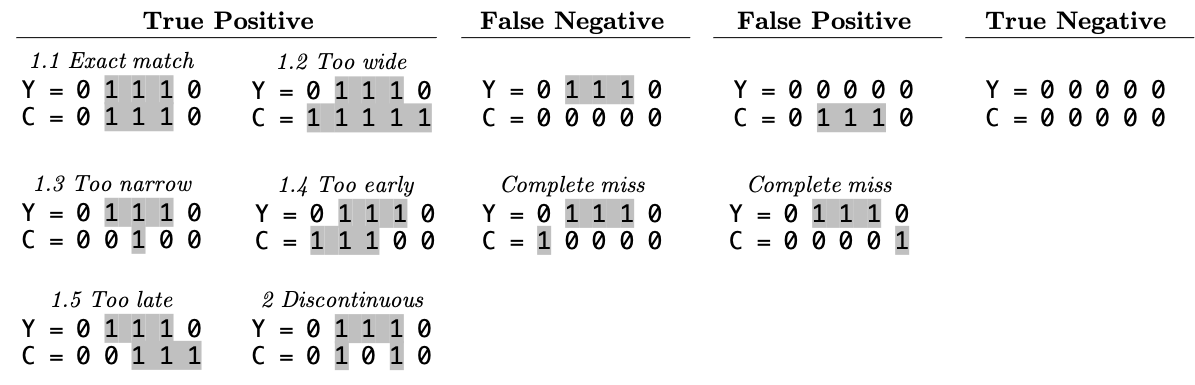
\includegraphics[scale=0.66]{prediction types}
\caption{Different types of predictions at the scope level. Note: Y denotes the vector of true scope labels, C denotes its classification vector. These are hypothetical examples for a sentence with 5 tokens.}
\label{scopelevel}
\end{figure*}

\subsection{Performance evaluation}
The performance of the model was evaluated at the token level and at the sentence level, and compared to existing methods when possible. At the token level, precision, recall and the $F_1$-measure were used as indicators of performance\footnotemark, that is, the performance on classifying a single token to be inside or outside of the negation scope. To this end, a classification vector $\mathbf{p}_i = (p_{1_i}~\cdots~p_{n_i})^{\prime}$ for sentence $s_i$ is element-wise compared to the label vector $\mathbf{y}_i$, where the classification $p_{t_i}$ equals 1 if $\pi_{t_i}\ge.5$ and 0 if $\pi_{t_i}<.5$. 

\footnotetext{Precision is defined as $\frac{\mathrm{tp}}{\mathrm{tp}+\mathrm{fp}}$, recall as $\frac{\mathrm{tp}}{\mathrm{tp}+\mathrm{fn}}$ and $F_1$ as $\frac{2\cdot\mathrm{precision}\cdot\mathrm{recall}}{\mathrm{precision}+\mathrm{recall}}$, where tp = true positives, fp = false positives and fn =  false negatives}

At the sentence level, a classification vector is regarded a true positive if it contains at least one true positive prediction at the token level, following the guidelines of the *SEM Shared Task 2012 \citep{SEM-shared-task}. This is the case when there is a negation scope, and at least one of the scope tokens is detected. False negatives are those instances where there is a negation scope, but none of the scope tokens is detected. True negatives are those instances where a sentence does not contain a negation scope, and the classification vector predicts no negation scope. Finally, false positives are those instances where each \textit{positive} prediction at the token level is a false positive, regardless of whether there is a negation scope. A special case is when there is a negation scope, the classification vector predicts a scope but none of the true negation tokens are detected. This is referred to as a \textit{complete miss}. 

To gain more insight into the true positives, which include any partially correct prediction, a distinction is made between (1) continuous scope predictions and (2) discontinuous scope predictions. A discontinuous scope prediction is a classification vector that contains the sequence $(1~0^{*}~1)^{\prime}$, where $0^{*}$ denotes a sequence of one or more zeros. The continuous scope predictions are further divided into (1.1) exact scope matches, and scope predictions that are (1.2) too wide, (1.3) too narrow, (1.4) too early or (1.5) too late. See Figure \ref{scopelevel} for an overview of all types of predictions at the scope level.

At the scope level, too, precision, recall and the $F_1$-measure were computed.

\section{Results}

\begin{table*}[t]
\caption{Model performance at the token level and the scope level.}
\label{allresults}
	\centering
	\begin{tabular}{l c | c c c c c | c c c}
	\hline
	Study & Level & Total & tp & fn & tn & fp & P(\%) & R(\%) & $F_1$ \\
	\hline \hline
	
	\multirow{2}{*}{Current} & Tokens & 70,496 & 2,575 & 874 & 66,405 & 642 & 80.0 & 74.7 &  77.3 \\
	 & Scopes & 2962 & 405 & 13 & 2544 & 0 & 100.0 & 96.9 & 98.4 \\
	\hline
	
	\multirow{2}{*}{\cite{fancellu2016neural}} & Tokens & 1,830 & 1,570 & 260 & - & 157 & 90.9 & 85.8 &  88.3 \\
	 & Scopes & - & - & - & - & - & 99.4 & 60.8 & 75.5 \\
	\hline
	
	\multirow{2}{*}{\cite{sergeeva2019}} & Tokens & - & - & - & - & - & 85.4 & 90.8 &  87.9 \\
	 & Scopes & - & - & - & - & - & - & - & - \\
	\hline
	
	\multirow{2}{*}{\cite{zou-etal-2013-tree}} & Tokens & - & - & - & - & - & 93.8 & 91.9 &  92.9 \\
	 & Scopes & - & - & - & - & - & - & - & - \\
	\hline
	
	\multirow{2}{*}{\cite{ozgur-radev-2009-detecting}} & Tokens & - & - & - & - & - & 75.8 & 90.8 &  82.6 \\
	 & Scopes & - & - & - & - & - & - & - & - \\
	\hline
	
	\end{tabular}
	\caption*{Note: P = Precision, R = Recall, tp = true positives, fn =  false negatives, tn = true negatives and fp = false positives, - = Not available.} 
\end{table*}

The model performs reasonably well at the token level: The precision is 80.0\%, the recall is 74.7\% and the $F_1$ is 77.3\%. At the scope level, the model performs very well: The precision is 100.0\%, the recall is 96.9\% and the $F_1$ is 98.4\%, see Table \ref{allresults}. Furthermore, none of the false negatives were complete misses. Most of the true positives (43.5\%) are exact matches, see Table \ref{tpresults}.

\begin{center}
\captionsetup{type=table}
	\caption{Distribution of true positives at the scope level.}
	\label{tpresults}
	\begin{tabular}{l | c}
	\hline
	Type of true positive & Percentage  \\
	\hline \hline
	1.1 Exact matches & 43.5\% \\
	1.2 Too wide & 27.9\% \\
	1.3 Too narrow & 22.7\% \\
	1.4 Too early & 0\% \\
	1.5 Too late & 4.7\% \\
	2 Discontinuous & 1.2\% \\
	\hline
	\end{tabular}
\end{center}

\section{Discussion}

The current study uses a BiLSTM-based model to detect negation scopes in biomedical text data with negated and non-negated sentences, generalizing the method proposed by \citep{fancellu2016neural}. Moreover, the study prevents overfitting negation scopes enclosed by punctiation marks. In this way, it contributes to the question of how negation scopes can be automatically resolved by Neural Network-based methods.

Intermediate results suggest that the proposed model achieves an excellent performance at the scope level. Note, however, that differences among studies in defining scope level performance makes comparisons problematic. Some studies only provide the percentage of correctly identified scopes, or no metric at all. 

It could be argued that the scope level is more relevant than the token level, since negation cues affects the meaning of a word sequence, rather than the meaning of words on their own. Therefore, the current study proposed some additional metrics at the scope level to gain more insight in the predictions at this level. To expand this effort, the boundaries of negation scopes could be inspected more closely with, for example, boundary measures used by \cite{qian-etal-2016-speculation}. 

At the token level, the model underperforms compared to state-of-the-art methods, see Table \ref{allresults}. There are multiple stategies to improve model performance at this level. First, experiments with different hyperparameter settings could improve the performance of the model. For example, the threshold of a positive prediction could be decreased, given the fact that the recall is rather low at the token level and many of the scope predictions were too wide. Second, the scope predictions could be improved by applying a `continuizer' to them, given the fact that all true scopes are continuous. This could be a simple rule that converts discontinuous scope segments $(1~0*~1)^{\prime}$ to $(1~1*~1)^{\prime}$. For the current model, discontinuous scope predictions are not common, but these may be more prevalent with a lower threshold setting. Third, the model can benefit from external information. For example, a part-of-speech tagger could be added to provide the model with more syntactic information, following \cite{sergeeva2019} and \cite{fancellu2016neural}. Also, model performace might improve by using pre-trained word embeddings, for example, contextualized word embeddings from ELMo \citep{ELMo}, and possibly update the embeddings given the current task. 

Finally, there are two interesting ways to extend the current study. First, information about the negation cues can be predicted from a preceding part of the model. This is consistent with the goal to be less dependent on manually-crafted features, but may decrease model performance, since cue predictions are not likely to be perfectly accurate. Second, the BioScope corpus is provided with speculation scope annotations, so it would be interesting to evalute whether the current model is generalizable to detection of this linguistic phenomenon as well.

\end{multicols}

\newpage
\bibliographystyle{apacite}
\bibliography{refs_report}

\end{document}
 